\chapter{Automatische Spracherkennung}

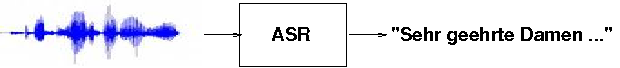
\includegraphics[width=\textwidth]{grafiken/automatische-spracherkennung/block.png}


\section{Stichworte zum Vortrag \em{Automatische Spracherkennung}}

Frontend, Backend, bottom-up, top-down, Merkmalsvektor, Variabilität von Sprachsignalen, Störparameter

\section{Literatur}

        {\em Gute Einführung:}\\
%        Euler S (2006): Grundkurs Spracherkennung. Vieweg Wiesbaden.\\
        Pfister, B. \& Kaufmann, T. (2008). Sprachverarbeitung - Grundlagen und 
	Methoden der Sprachsynthese und Spracherkennung. 
	Springer-Verlag Berlin Heidelberg.

%        {\em Die Verwendung von ANN in der ASR:}\\
%	Bourlard H, Morgan N (1994): Connectionist Speech Recognition - 
%	A Hybrid 
%	Approach Kluwer Academic Publishers, Engineering and Computer 
%	Science.
%       {\em Beispiel für eine spezielle Merkmalsextraktion:}\\
%	Hermansky H, Morgan N, Bayya A, Kohn P (1991): Compensation for 
%	the Effect of the Communication Channel in Auditory-Like Analysis 
%	of Speech (RASTA-PLP), EUROSPEECH 1991, Genua, p. 1367 - 1370.

 %       {\em Grundlegender Artikel über das Viterbi-Training von HMM:}\\
%	Juang B H, Rabiner L R (1990): The segmental k-means algorithm for 
%	estimating parameters of Hidden Markov Models.
%	IEEE Transactions on Acoustics, Speech and Signal Processing, Vol. 38, 
%	No. 9, Sep 1990, S. 1639 - 1641.	

        {\em Einführung in ANN:}\\
	Lippmann, R. S. (1987). An Introduction to Computing with Neural Nets.
	IEEE. ASSP Magazine. April 1987. S.\,4 - 22.

%        {\em Einführung über Dynamic Time Warping als Mustererkennung:}\\
%	Ney H, Ortmanns S (1999): Dynamic Programming Search for 
%	Continuous Speech Recognition. in: IEEE Signal Processing Magazine, 
%	Sept 1999, pp. 64-83.

 %       {\em Gute Einführung in HMM in der ASR:}\\
%	Picone J (1990): Continuous Speech Recognition Using Hidden Markov Models.
%	IEEE ASSP Magazine, Jul 1990, S. 26 - 41.

 %       {\em Grundlegender Artikel über HMM:}\\
%	Rabiner L R, Juang B H (1996): An Introduktion to Hidden Markow Modells
%	IEEE ASSP Magazine, Jan 1986, p. 4.

%	{\em Einführendes Buch über Akustische Phonetik; Kapitel 2.4 - 2.8 sind 
%	sehr gute Erklärungen zum digitalen Signal und Spektrum:}\\
%	Reetz H (2003): Artikulatorische und akustische Phonetik, 
%	Wissenschaftlicher Verlag Trier.

        {\em Gutes Lehrbuch über alle Arten von Sprachverarbeitung:}\\
        Jurafsky D. \& Martin J. H. (2000). Speech and Language Processing. 
	Prentice Hall. Kap I.7.

%        {\em Mathematische Theorie der Spracherkennung; ziemlich schwierig; 
%	interessant (auch ohne viel Mathe-Kenntnisse): Kapitel 7:}\\
%        Levinson S (2005): Mathematical Models for Speech Technology, John Wiley \& Sons, UK.

%        {\em Wissenschaftliches Arbeiten:}\\
%        Bördlein S (2002): Das Sockenfressende Monster in der Waschmaschine. Alibri Verlag Gunnar Schedel.
